\section{Khuur үр дүн}
\subsection{Нүүр хэсэг}

\begin{figure}
	\centering
	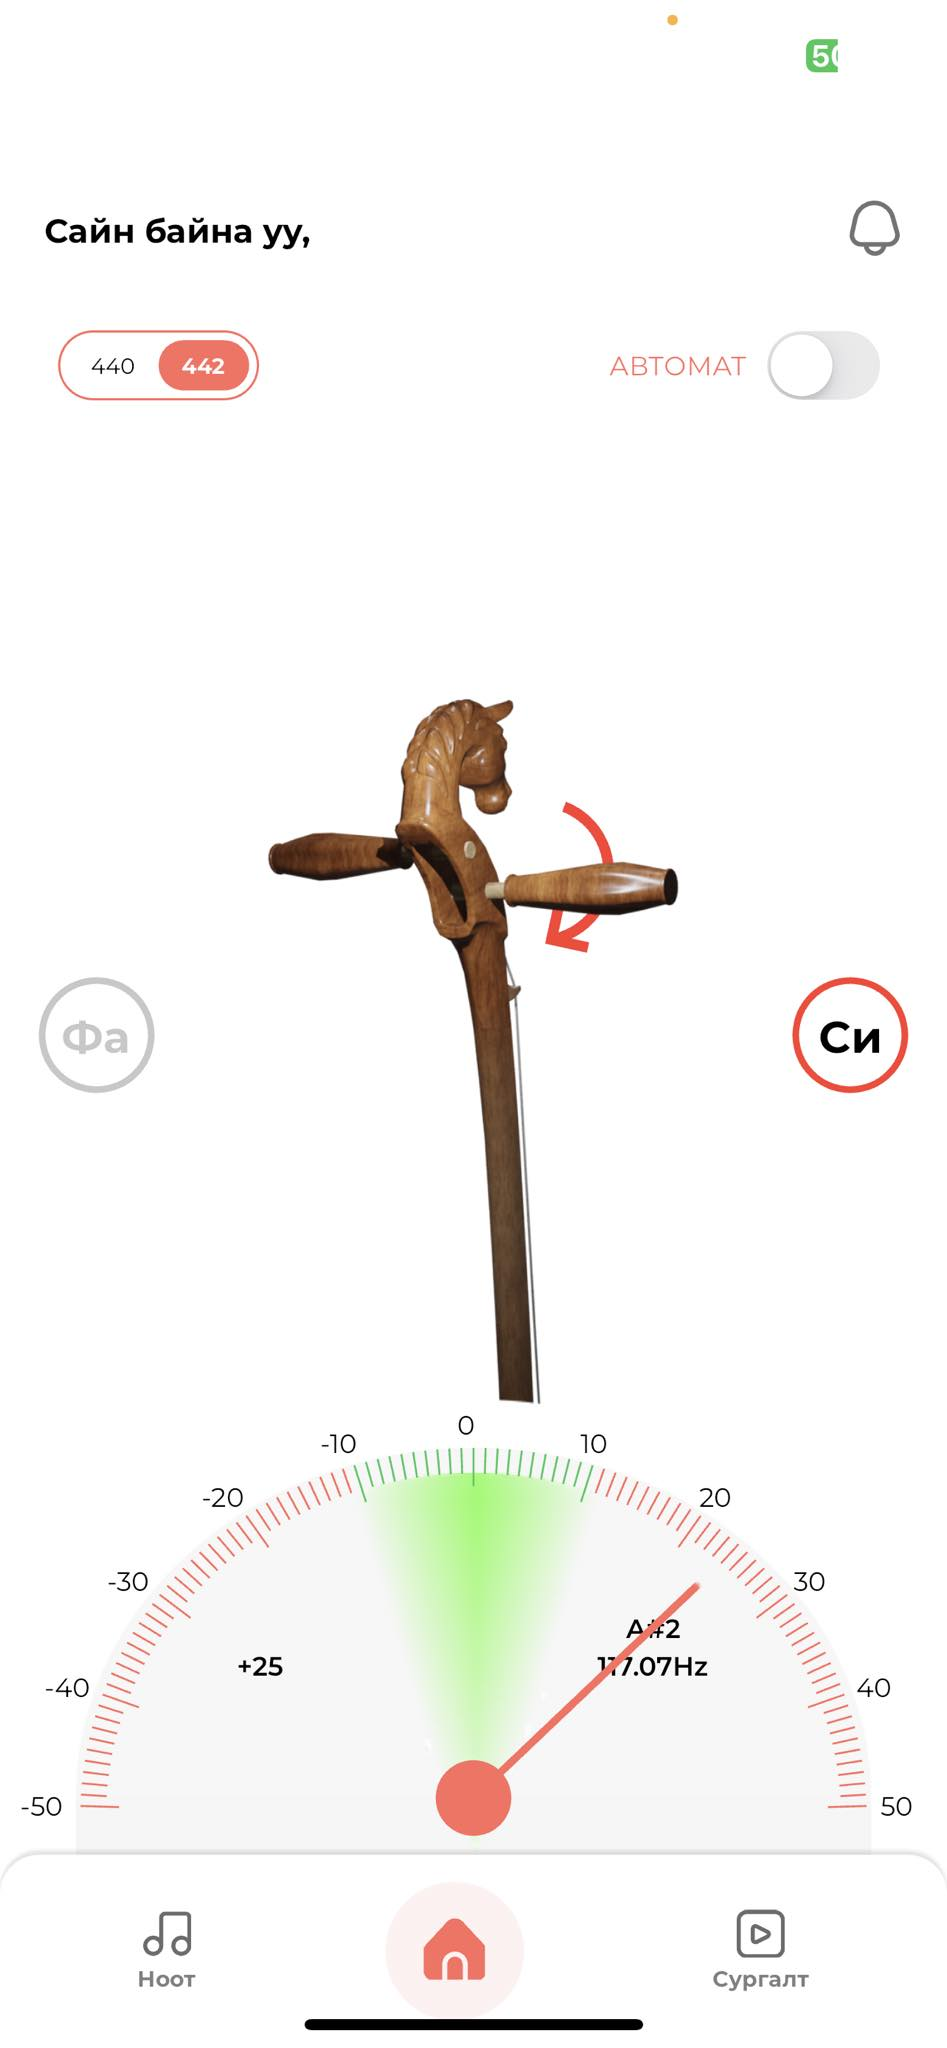
\includegraphics[height=15cm]{images/khuur-app1.jpg}
	\caption{Нүүр хэсэг}
	\label{fig:homepage}
\end{figure}
\pagebreak

\subsection{Түр хүлээгдэж буй хуудасны загвар}

\begin{figure}[h]
	\centering
	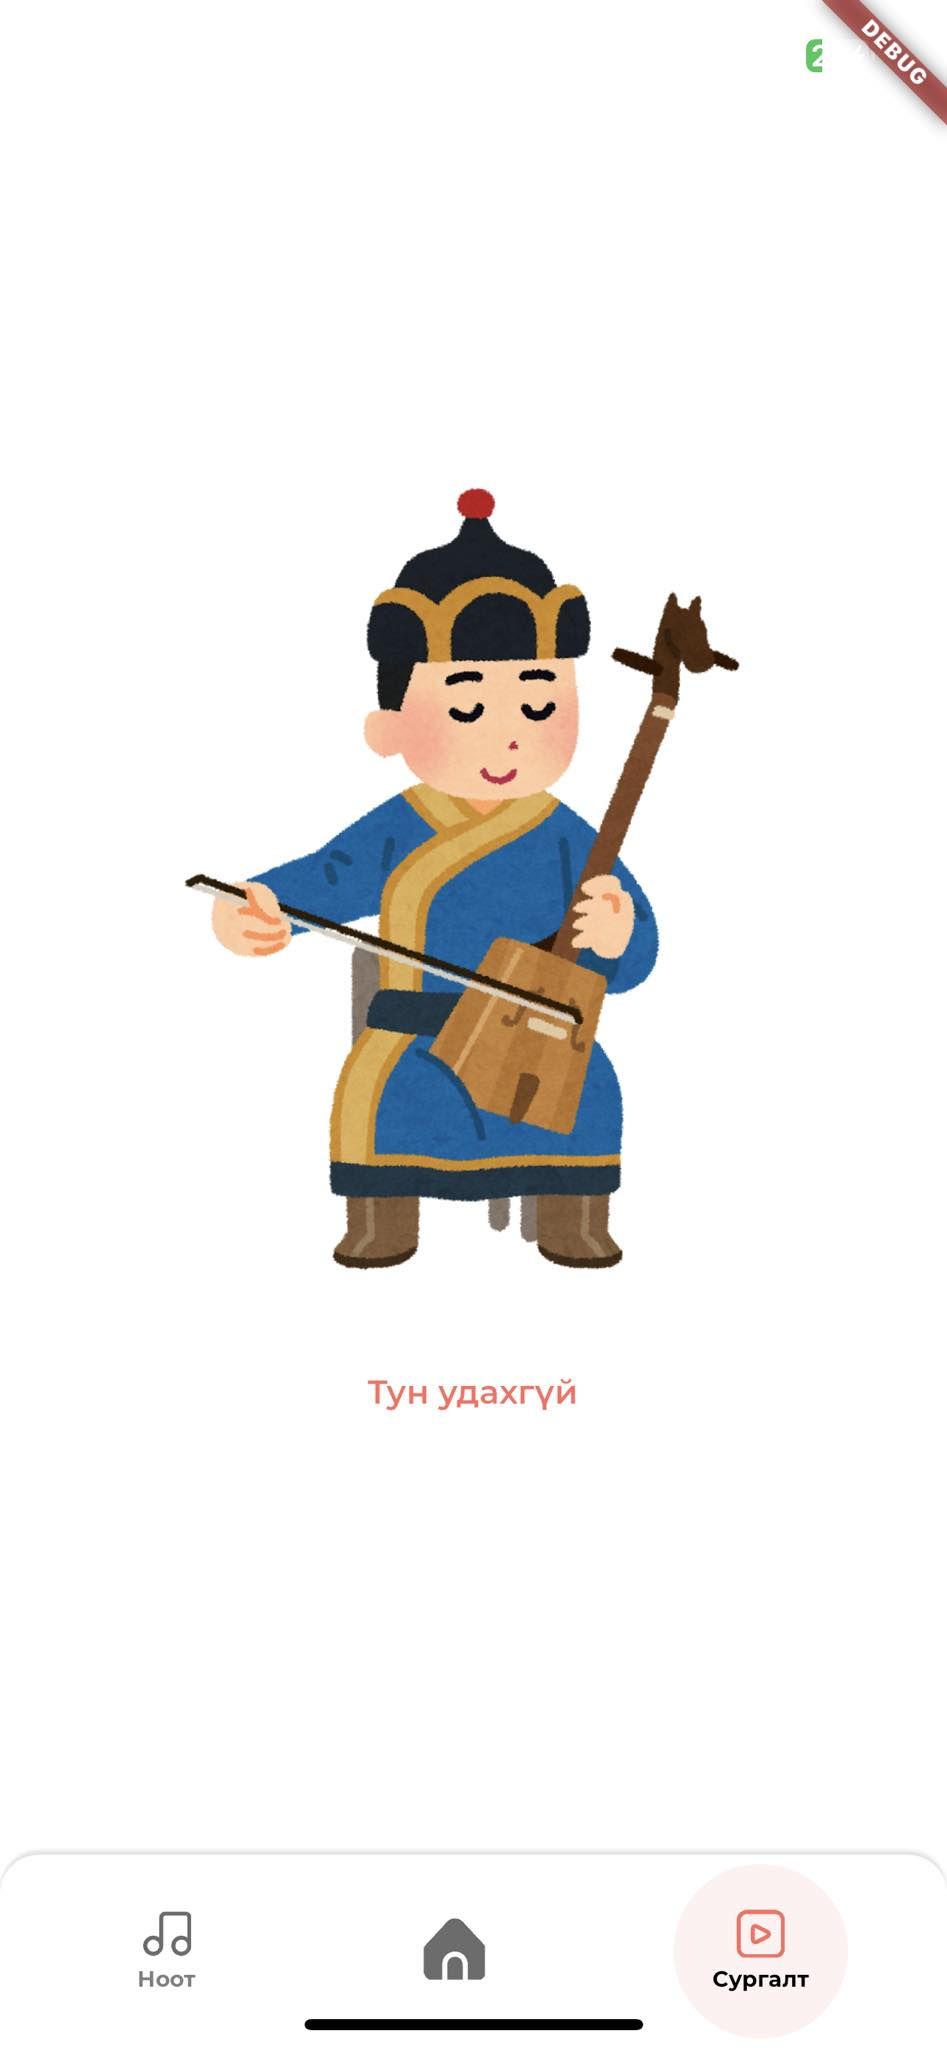
\includegraphics[height=15cm]{images/khuur-app2.jpg}
	\caption{"Тун удахгүй" хуудас}
	\label{fig:modalform}
\end{figure}
\pagebreak

\section{Data Spider үр дүн}

\subsection{Нэвтрэх хэсэг}
\begin{figure}
	\centering
	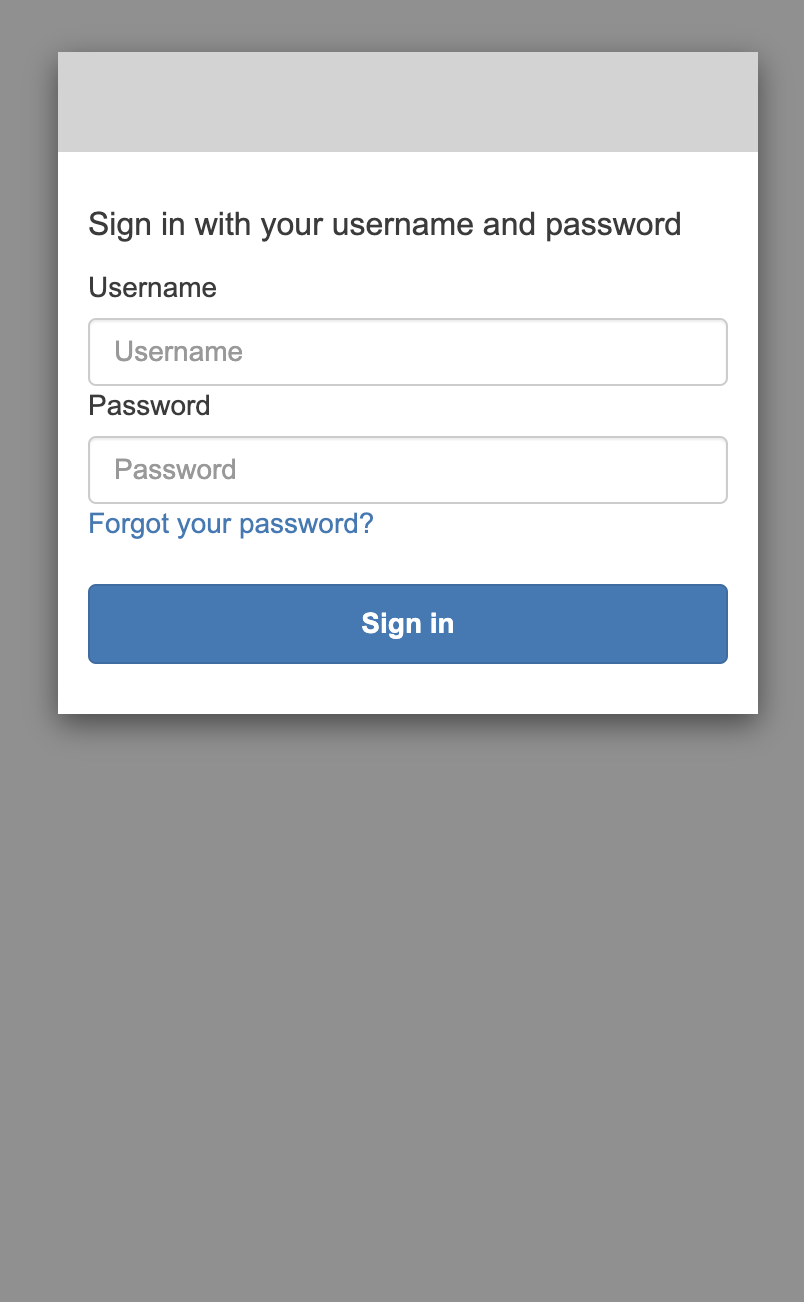
\includegraphics[height=15cm]{images/dataspider-login.png}
	\caption{Data Spider нэвтрэх хуудас}
	\label{fig:toast}
\end{figure}
\pagebreak
\subsection{Нэвтрэх хэсэг}
\begin{figure}[h]
	\centering
	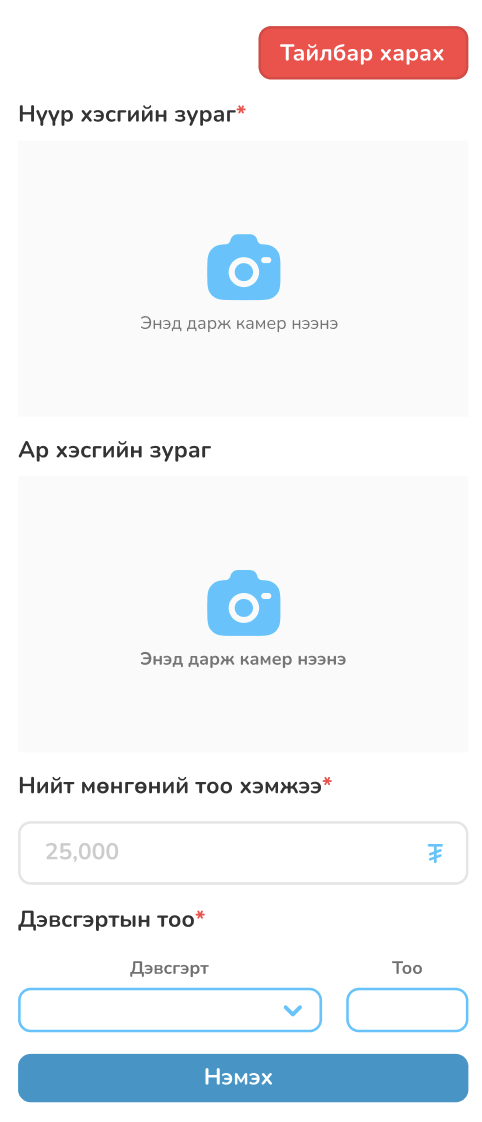
\includegraphics[height=15cm]{images/dataspider.png}
	\caption{Data Spider нүүр хуудас}
	\label{fig:toast}
\end{figure}
\pagebreak
\pagebreak
\section{Үр дүнгийн тайлан}
Миний бие Отгонбаатар овогтой Цэнгүүн нь 1 сарын хугацаанд ХандПро компанид үйлдвэрлэлийн дадлагаа амжилттай дүүргэлээ. Богинохон хугацаанд сурч мэдэж авсан онолын мэдлэг чадвараа практик дээр ашиглаж туршлага хуримтлуулж, сурахыг хүсэж байсан олон технологиудаа судалж, мундаг мэргэжилтнүүдээс бодит зөвлөгөө авсан үр дүнтэй туршлага боллоо. Программм хангамжийн бүтээгдэхүүний шаардлага тодорхойлохоос эхлээд PlayStore дээр байршуулж хэрэглэгчийн гарт хүргэх хүртэлх процессуудын үе шат бүхэнд оролцлоо. Flutter болон АWS технологийн талаарх сайн ойлголттой болж бие дааж бүтээгдэхүүн хөгжүүлэх урам зориг авлаа. Мөн жижиг стартап компанийн ажлын орчин, арга барил, болон зах зээлийн бодит амьдралыг биеэрээ мэдэрч суралцаж цаашдаа энэ замналаар нийгэмд хэрэгцээтэй шийдэл санаа хөгжүүлэх сэдлийг төрүүллээ.